\documentclass[a4paper,11pt]{jsarticle}


% 数式
\usepackage{amsmath,amsfonts, amssymb}
\usepackage{bm}
% 画像
\usepackage[dvipdfmx]{graphicx}


\begin{document}

\title{巡回符号の課題}
\author{}
\date{\today}
\maketitle


\section{$n=5$の巡回符号}
生成多項式$g(x)$は$1+x^n$の因数なので、
\[
  1+x^5=(1+x)(1+x+x^2+x^3+x^4)
\]
より、$g(x)$の候補は$1+x$と$1+x+x^2+x^3+x^4$
である。
$g(x)=1+x$のときの全ての符号を表\ref{table:n5g1}
に示す。
\begin{table}[hbtp]
  \caption{$g(x)=1+x$の符号}
  \label{table:n5g1}
  \centering
  \begin{tabular}{ccccc}
    00000 &&&& \\
    00011 & 00110 & 01100 & 11000 & 10001 \\
    00101 & 01010 & 10100 & 01001 & 10010 \\
    01111 & 11110 & 11101 & 11011 & 10111
  \end{tabular}
\end{table}
表\ref{table:n5g1}より、$g(x)=1+x$のときの最小ハミング距離は2である。
$g(x)=1+x+x^2+x^3+x^4$のとき、符号は00000と11111のみなので、
最小ハミング距離は5である。

\section{$n=6$の巡回符号}
生成多項式$g(x)$は$1+x^n$の因数なので、
\[
  1+x^6=(1+x^3)^2=(1+x)^2(1+x+x^2)^2
\]
より、$g(x)$の候補を$k$の昇順に並べると
表\ref{table:n6g}になる。
\begin{table}[hbtp]
  \caption{$n=6$の巡回符号の生成多項式}
  \label{table:n6g}
  \centering
  \begin{tabular}{c|l}
    $k$ & $g(x)$ \\ \hline
    1 & $(1+x)(1+x+x^2)^2$ \\
    2 & $(1+x+x^2)^2$ \\
    2 & $(1+x)^2(1+x+x^2)$ \\
    3 & $(1+x)(1+x+x^2)$ \\
    4 & $1+x+x^2$ \\
    4 & $(1+x)^2$ \\
    5 & $1+x$
  \end{tabular}
\end{table}

\section{$g(x)=(1+x)(1+x^2+x^3)$の巡回符号の生成行列}
$n=7$の場合、$g(x)$の次数が4なので、情報源の長さは3である。
$g(x)$を展開すると$1+x+x^2+x^4$となり、
生成行列は1行目が$x^2g(x)$, 2行目が$xg(x)$, 3行目が$g(x)$
になるので、
\[
  {\bm G}=
  \begin{bmatrix}
    0 & 0 & 1 & 1 & 1 & 0 & 1 \\
    0 & 1 & 1 & 1 & 0 & 1 & 0 \\
    1 & 1 & 1 & 0 & 1 & 0 & 0
  \end{bmatrix}
\]
となる。これを組織符号に変換すると
\[
  \begin{bmatrix}
    0 & 1 & 1 \\
    1 & 1 & 0 \\
    1 & 0 & 0
  \end{bmatrix}
  \begin{bmatrix}
    0 & 0 & 1 & 1 & 1 & 0 & 1 \\
    0 & 1 & 1 & 1 & 0 & 1 & 0 \\
    1 & 1 & 1 & 0 & 1 & 0 & 0
  \end{bmatrix}=
  \begin{bmatrix}
    1 & 0 & 0 & 1 & 1 & 1 & 0 \\
    0 & 1 & 0 & 0 & 1 & 1 & 1 \\
    0 & 0 & 1 & 1 & 1 & 0 & 1
  \end{bmatrix}
\]

\section{$g(x)=1+x^2+x^3$の(7,4)巡回符号}
\subsection{符号化回路とその動作}
$g(x)=1+x^2+x^3$の(7,4)巡回符号の符号化回路
を図\ref{fig:encoding-circuit}に示す。
\begin{figure}[htbp]
  \begin{center}
  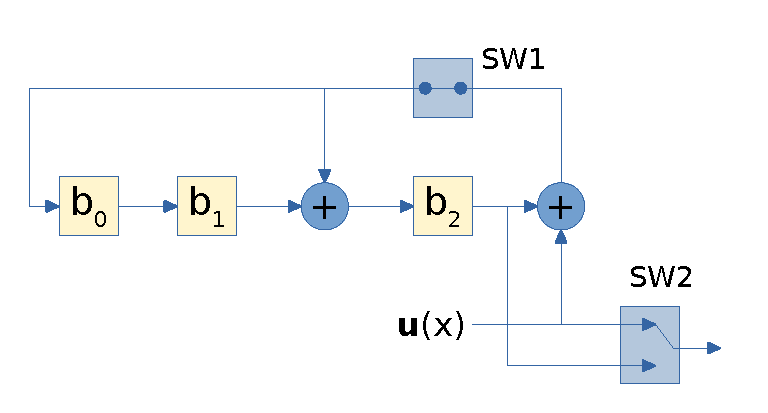
\includegraphics[scale=1.0]{figures/cyclic7-4-encoding.pdf}
  \end{center}
  \caption{符号化回路
  \label{fig:encoding-circuit}
  }
\end{figure}
この回路に入力情報$u(x)=1+x^2$を
入れたときの動作を表\ref{table:circuit-behavior}に示す。
情報の長さは4なので、入力の順番は0101である。
\begin{table}[hbtp]
  \caption{$u(x)=1+x^2$を入れたときの動作}
  \label{table:circuit-behavior}
  \centering
  \begin{tabular}{cc|ccc|c}
    & 入力 & $b_0$ & $b_1$ & $b_2$ & 出力 \\ \hline
    & - & 0 & 0 & 0 & - \\
    & 0 & 0 & 0 & 0 & 0 \\
    SW1: 閉 & 1 & 1 & 0 & 1 & 1 \\
    SW2: 上 & 0 & 1 & 1 & 1 & 0 \\
    & 1 & 0 & 1 & 1 & 1 \\ \hline
    SW1: 開 & - & 0 & 0 & 1 & 1 \\
    SW2: 下 & - & 0 & 0 & 0 & 1 \\
    & - & 0 & 0 & 0 & 0
  \end{tabular}
\end{table}

\subsection{シンドローム計算回路}
シンドローム計算回路を図\ref{fig:calc-syndrome-circuit}に示す。
\begin{figure}[htbp]
  \begin{center}
  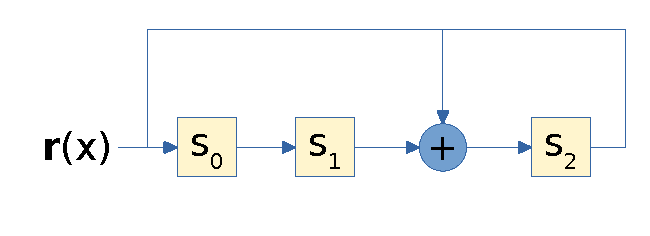
\includegraphics[scale=1.0]{figures/calc-syndrome-cyclic-7-4.pdf}
  \end{center}
  \caption{シンドローム計算回路
  \label{fig:calc-syndrome-circuit}
  }
\end{figure}
受信語が$r(x)=x^2+x^4+x^5$の場合の
回路の動作を表\ref{table:syndrome-behavior}に示す。
\begin{table}[hbtp]
  \caption{$r(x)=x^2+x^4+x^5$を入れたときの動作}
  \label{table:syndrome-behavior}
  \centering
  \begin{tabular}{c|ccc}
    入力 & $s_0$ & $s_1$ & $s_2$ \\ \hline
    - & 0 & 0 & 0 \\
    0 & 0 & 0 & 0 \\
    1 & 1 & 0 & 0 \\
    1 & 1 & 1 & 0 \\
    0 & 0 & 1 & 1 \\
    1 & 0 & 0 & 0 \\
    0 & 0 & 0 & 0 \\
    0 & 0 & 0 & 0
  \end{tabular}
\end{table}
シンドロームが最終的に0になったので誤りなし。
また、$r(x)=x^2g(x)$であることからも、
誤りがないことが分かる。

\section{$g(x)=1+x+x^4$の(15, 11)ハミング符号}
符号化回路を図\ref{fig:hamming15-11-encoding}に示す。
\begin{figure}[htbp]
  \begin{center}
  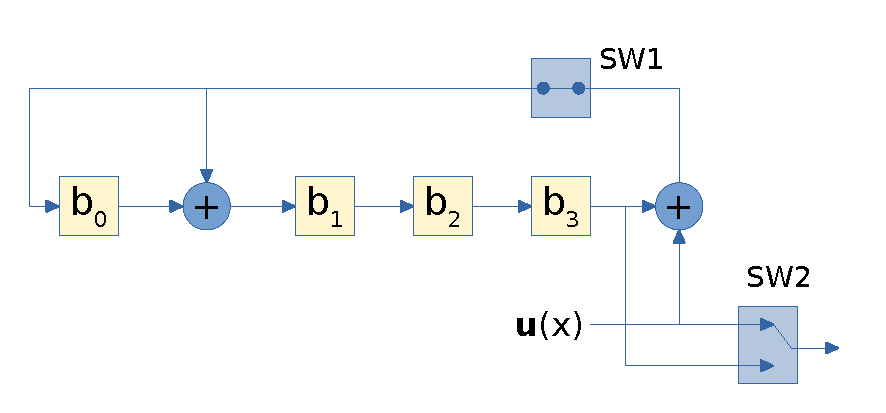
\includegraphics[scale=1.0]{figures/hamming15-11-encoding.pdf}
  \end{center}
  \caption{$g(x)=1+x+x^4$の(15, 11)ハミング符号の符号化回路
  \label{fig:hamming15-11-encoding}
  }
\end{figure}

\end{document}